\chapter{Mathematical background}
The flow of CSF around the spinal cord requires equations for fluid flow to be coupled with equations for elasticity or in the optimal case, poroelasticity. The underlying concepts of these kinds of problems were originally developed somewhat independently within petroleum engineering, geomechanics and hydrogeology. The equations will first be presented separately. Later in the chapter, coupling conditions will be discussed. Several quantities will be discussed and we try to use a consistent notation for each quantity throughout the study. 
\\
\\
This chapter intends to give a short description of the mathematical theory behind modeling of CSF. The equations are first introduced by assuming a fixed set of coordinates. Later, the two fundamental descriptions of motion are discussed. \\
\\
In this thesis we use the following notation for the physical quantities: \\ \\
$\mathbf{v}$ - Velocity of the material. In the fluid, $\mathbf{v}$ represents fluid velocity, and in the solid $\mathbf{v}$ denotes the velocity of the solid.
\\ \\
$ \mathbf{U}$ - Total displacement of the solid. In the fluid, this quantity represents the total mesh displacement. 
\\
\\
$p$ - Pressure in the fluid. In the case of elasticity, the same pressure does not exist in the solid, but in the case of an (almost) incompressible solid, an extra equation involving $p$ can be set up in the solid as well. 
\\
\\
$\mathbf{w}$ - Domain velocity, (i.e, all material points within the domain moves with velocity $\mathbf{w}$). In the solid, the domain changes with the velocity of the solid, $\mathbf{v}$, so in the solid we have $\mathbf{v} = \mathbf{w}$ which will not neccessary hold in the fluid.
\\
\\
Subscripts f and s are used to denote fluid and solid quantities, respectively
\section{Fluid flow}
The most fundamental equations in fluid flow are conservation laws. These equations are based on classical mechanics and states conservation of mass, momentum and energy. In the literature, these are often reffered to as balance equations.

\subsection{Reynolds Transport Theorem}
The famous engineer and scientist Osbourne Reynold stated the general conservation law the following way \cite{Reyn1903}:
\\
\\
Any change whatsoever in the quantity of any entity within a closed surface can only be effected in one or other of two distinct ways:
\begin{enumerate}
\item it may be effected by the production or destruction of the entity within the surface, or
\item by the passage of the entity across the surface.
\end{enumerate}
\begin{center}
\begin{figure}[!ht]
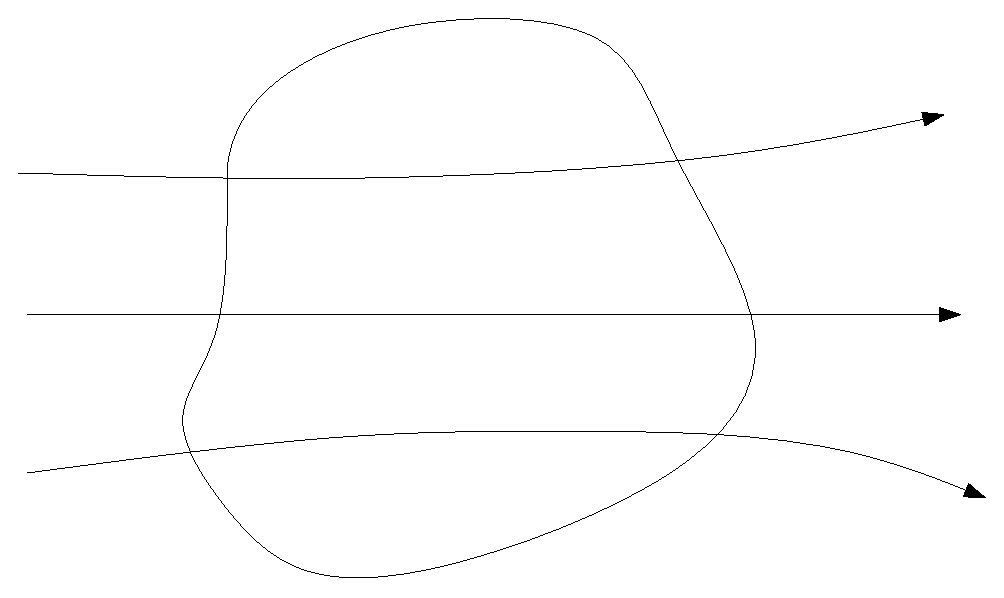
\includegraphics[scale=0.5]{figures/Fixed_control_volume} \\
\caption{Fixed control volume with flow as indicated by streamlines} 
\end{figure}
\end{center}
It should be noted that the transport theorem can be approached in two different ways. One for a fixed set of spatial coordinates, a fixed control volume, where fluid can enter and exit the boundaries of the defined body. The other approach has a control volume consisting of the same material particles at all times. Therefore the body has to follow the flow, and no fluid will cross the boundary. In this approach, one has to take into account the movement of the boundary of the body and the fact that the body can change it's volume. More on descriptions of motion is described in section \ref{sec:DoM}
\begin{center}
\begin{figure}[!ht]
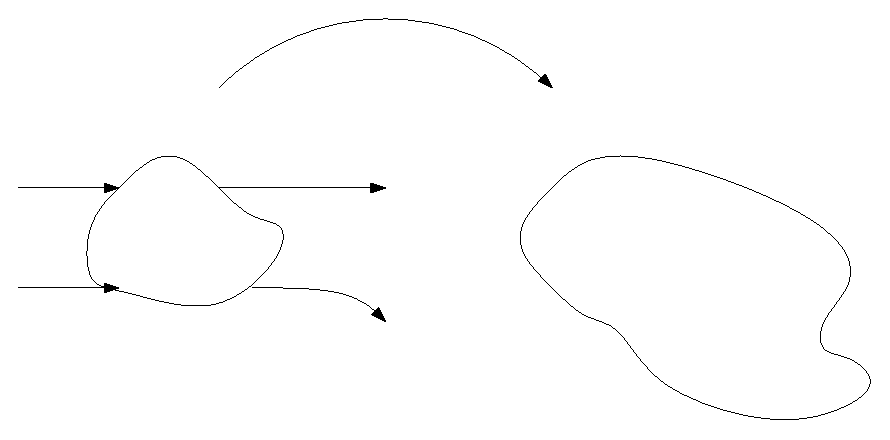
\includegraphics[scale=0.8]{figures/Moving_control_volume}\\
\caption{A moving control volume, consisting of the same fluid particles at time $t$ (left) and time $t+\Delta t$ (right) }
\end{figure}
\end{center}
Now, consider a fixed control volume, $V_0$ and some fluid property $Q(\mathbf{x},t)$. The rate of change of $Q$ within the control volume can be written
\begin{align}
\frac{\mathrm{d}}{\mathrm{d}t} \int_{V_0} Q(\mathbf{x},t) \, \mathrm{d}V \label{Rate_of_change}
\end{align}
The net change of $Q$ must be equal the rate of change in $Q$ within the control volume plus the net rate of mass flow out of the volume. In other words:
\begin{align}
\frac{\mathrm{d}}{\mathrm{d}t} \int_{V_0} Q(\mathbf{x},t) \, \mathrm{d}V = \int_{V_0} \pdi{Q(\mathbf{x},t)}{t} \mathrm{d}V + \int_{S_0} Q(\mathbf{x},t) \mathbf{v} \cdot \mathbf{n} \mathrm{d}S \label{Reynolds}
\end{align}
Here, $\mathbf{v}$ denotes fluid velocity, and $\mathbf{n}$ denotes the outward pointing unit-normal, i.e $\mathbf{n}$ points \textit{out} of the fluid. This equation is known as the Reynold's transport theorem. The right hand side could be rewritten by using Gauss' theorem on the last term. 
\begin{align}
\frac{\mathrm{d}}{\mathrm{d}t} \int_{V_0} Q(\mathbf{x},t) \, \mathrm{d}V = \int_{V_0} \big{[}\pdi{Q(\mathbf{x},t)}{t} + \nabla \cdot (Q(\mathbf{x},t) \mathbf{v}) \big{]}\mathrm{d}V \label{Reynold}
\end{align}
where \[ \nabla = \mathbf{i}_j\pdi{}{x_j} \]
\subsection{Conservation of mass and momentum}
Choose $Q(\mathbf{x},t) = \rho$. Conservation of mass means that
\begin{align*} 
\frac{\mathrm{d}}{\mathrm{d}t} \int_{V_0} \rho \, \mathrm{d}V = 0
\end{align*}
And by using the transport theorem \eqref{Reynold}
\begin{align}
\int_{V_0} \big{[}\pdi{\rho}{t} + \nabla \cdot (\rho \mathbf{v}) \big{]}\mathrm{d}V = 0
\end{align}
This should hold for any volume $V_0$, hence the integrand has to be zero. If there existed a point where the integrand were not zero, the control volume could be an arbitrary small enclosed sphere around this point, and the volume integral would not be zero. Therefore, 
\begin{align} 
\pdi{\rho}{t} + \nabla \cdot (\rho \mathbf{v}) = 0 \label{Continuity}
\end{align}
\eqref{Continuity} is known as the continuity equation and states conservation of mass. 
\\
\\
To derive a simliar property for the momentum, Newtons second law of motion can be used. The net change of momentum must be equal to the applied forces to the system. The forces can be divided into volume forces, acting on the entire control volume, and forces acting only on the control surface. The forces acting on the surface can be written $\sigma_f \cdot \mathbf{n}$, where $\sigma_f = \sigma_f(\mathbf{v}, p)$ is the tensor denoting the total stress. \\
\\
This can be written
\begin{align*} \frac{\mathrm{d}}{\mathrm{d}t} \int_{V_0} \rho \mathbf{v}(\mathbf{x},t) \mathrm{d}V = \int_{\partial V_0}\sigma_f \cdot \mathbf{n} \,\mathrm{d}S + \int_{V_0} \mathbf{F}_v \mathrm{d}V
\end{align*}

By using the Transport Theorem on the left hand side and with Gauss' theorem on the right hand side we end up with
\begin{align*} \int_{V_0} [ \pdi{\rho \mathbf{v}}{t} + \nabla \cdot (\rho \mathbf{v}\mathbf{v} ) - \nabla \cdot \sigma_f - \mathbf{F}_v] \mathrm{d}V = 0
\end{align*}
With the same argument as before the integrand has to be zero, and with some rearrangement:
\begin{align}
\pdi{\rho \mathbf{v}}{t} + \nabla \cdot (\rho \mathbf{v}\mathbf{v} ) = \nabla \cdot \sigma_f + \mathbf{F}_v \label{M_0}
\end{align} 
The left hand side can be rewritten to
\begin{align}
\rho \pdi{\mathbf{v}}{t} + \mathbf{v} \pdi{\rho}{t} + \mathbf{v} \mathbf{v} \cdot \nabla \rho + \rho \mathbf{v} \cdot \nabla \mathbf{v} + \mathbf{v}\rho \cdot \nabla \mathbf{v} = \rho\Big{(}\pdi{\mathbf{v}}{t} + (\mathbf{v} \cdot \nabla ) \mathbf{v} \Big{)} + \Big{(}\pdi{\rho}{t} + \nabla \cdot (\mathbf{v} \rho)\Big{)}
\end{align}
And the last term is zero due to mass conservation. Equation \eqref{M_0} can then be written
\begin{align}
\rho \big{(}\pdi{\mathbf{v}}{t} + (\mathbf{v} \cdot \nabla ) \mathbf{v} \big{)} = \nabla \cdot \sigma_f + \mathbf{F}_v \label{Momentum}
\end{align} 

The stress tensor, $\sigma_f$, depends on fluid properties and will be defined in the next subsection. Equation \eqref{Momentum} is known as the momentum equation as it states conservation of momentum.
\\
\\
The energy equation for an incompressible flow is given by
\begin{align}
\rho c_p \pdi{T}{t} + \mathbf{v}\cdot \nabla T = k \nabla^2 T + \Phi \label{Energy}
\end{align}
Where $c_p$ is the heat capacity and $\Phi$ is the dissippation function. When $\rho$ and $\mu$ is constant, the other two balance equations, \eqref{Continuity} and \eqref{Momentum}, are uncoupled from the energy equation, and thus ignored from the set of equations. 
\subsection{Incompressible Newtonian fluids}
In this text we will only consider incompressible fluid flow for a Newtonian fluid. 
The assumption of a Newtonian fluid requires the viscous stresses to be linear functions of the components of the strain-rate tensor, denoted by $\epsilon$. These assumptions were first made by Stokes in 1845. Stokes' assumptions have later proven to be quite accurate for all gases and most common fluids. Stokes' three postulates regarding the deformation laws are: \cite{Whit06}
\begin{enumerate}
\item The fluid is continuous, and its stress tensor, $\sigma_{f_{ij}}$ is at most a linear function of the strain rates, $\epsilon_{ij}$ 
\item The fluid is isotropic, i.e., its properties are independent of direction, and therefore the deformation law is independent of the coordinate axes in which it is expressed. 
\item When the strain rates are zero, the deformation law must reduce to the hydrostatic pressure condition, $\sigma_{f_{ij}} = -p\delta_{ij}$, where $\delta_{ij}$ is the Kroenecker delta function. 
\end{enumerate}


From the first and third conition the following assumption can be made
\begin{align}
\sigma_{f_{ij}} = -p\delta_{ij} + M_{ijkl}\epsilon_{kl} \label{Hookes}
\end{align}
It can be shown that symmetry of $\sigma_f$ and $\epsilon$ also requires symmetry of $M$. This assumption reduces the number of coefficients in \eqref{Hookes} from 36 to 21. If Stokes' second condition is also taken into account and the fluid properties are identical in each direction the number of coefficients are further reduced to 2. These simplifications allow us to denote the stress tensor the following way:
\begin{align}
\sigma_{f_{ij}} = -p\delta_{ij} + 2\mu\epsilon_{ij} + \lambda \nabla \cdot \mathbf{v} \label{Stress}
\end{align}
where $\epsilon = \frac{1}{2}(\pdi{u_i}{x_j} + \pdi{u_j}{x_i})$, $p$ is the fluid pressure and $\mu$ and $\lambda$ are known as Lame's constants. In the present study we only consider incompressible flow where $\rho$ is constant. From the continuity equation \eqref{Continuity}, this implies $\nabla \cdot \mathbf{v} = 0$ and the last term in \eqref{Stress} vanishes. Furthermore, 
\begin{align*}
\nabla \cdot \epsilon = \pdi{}{x_j}(\pdi{u_j}{x_i} + \pdi{u_i}{x_j})\mathbf{i}_i = (\pdi{}{x_i}\pdi{u_j}{x_j} + \pdi{u_i}{x_j \partial x_j})\mathbf{i}_i = \pdi{u_i}{x_j \partial x_j} \mathbf{i}_i
\end{align*}
Which simplifies the representation of $\nabla \cdot \sigma_f$ in \eqref{Momentum} for an incompressible fluid

\subsection{Navier-Stokes equations for incompressible flow}
Stating both conservation of mass and momentum of a fluid together with suitable boundary conditions gives us all the information we need to be able to define the flow field and the corresponding pressure. This requires a solution to the system \eqref{Continuity}-\eqref{Momentum}, equations which are commonly referred to as the Navier-Stokes equations. With the simplifications described in the previous section the system of equations can be written
\begin{align}
\rho(\pdi{\mathbf{v}}{t} + (\mathbf{v} \cdot \nabla) \mathbf{v}) = -\nabla p + \mu\nabla^2 \mathbf{v} + \mathbf{F}_v \label{Navier}
\end{align}
\begin{align}
\nabla \cdot \mathbf{v} = 0 \label{Stokes}
\end{align}
The parameters $\rho$ and $\mu$ describe density and dynamic viscosity. Often, the momentum equation is written in terms of the kinematic viscosity $\nu = \frac{\mu}{\rho}$ by dividing the momentum equation with $\rho$. \\
These equations are coupled and non-linear and can generally not be solved analytically. However, numeruous analytical solutions have been carried out for different specific problems, and a good overview is given by White \cite[pp. 97-164]{Whit06}. (Further references are also given in this textbook for the interested reader) These problems are often very simple and idealized. Hence, numerical solutions are a necessity to obtain useful solutions to real-life problems. Such metods will be discussed in chapter xxx. 


\section{Linear Elasticity}
Linear elasticity is an approximation used for small deformations for elastic solids. As a rule of thumb the approximation of linear elasticity is usually valid for deformations up to 10\% relative to the solid. The stress tensor for a linear elastic medium is very similar to \eqref{Stress} describing an incompressible Newtonian fluid except there is no fluid pressure, and the stress is related to the total displacement $\mathbf{U}$ rather than the velocity $\mathbf{v}$. The stress tensor for such a material reads:
$\sigma_s = 2\mu\epsilon(\mathbf{U}) + \lambda \nabla \cdot \mathbf{U}$
\begin{align} 
\rho \pdi{^2\mathbf{U}}{t^2} = \nabla \cdot \sigma_s \label{LE}
\end{align}
The left hand side can also be expressed from the solid velocity $\mathbf{v}$ using that $\pdi{^2\mathbf{U}}{t^2} = \pdi{\mathbf{v}}{t} $. The advantage of using $\mathbf{v}$ as the unkown will be discussed in chapter xxx.
\\
Therefore, the governing equation for the Linear Elasticity problem will be
\begin{align}
\rho \pdi{\mathbf{v}}{t} = \nabla \cdot \sigma_s \label{LE2}
\end{align}
\section{Linear Poroelasticity}
In this section, the equations describing fluid flowing trough an elastic, porous medium is presented. For a more detailed discussion, derivation and history within the field we refer to \cite{Wang00} on Linear Poroelasticity. To keep the mathematics as similar to the fluid case as possible, we use $\mu$ and $\lambda$ instead of the possion ratio. The equations describing linear poroelasticity are often described as Biot's equations. 
\\
\\
\subsection{Fluid flow through a porous media}
A porous medium is a material with pores in which fluid can flow. The principles of modeling porous flow consist of macroscopic averaging over the pores. The material part is often known as the skeleton, matrix or frame and in general all the pores will have different size and shape. In this section the skeleton is assumed rigid. The nature of the material defines whether we will be able to fully solve the problem with no-slip conditions on all skeleton parts, or if some kind of volumetric averaging can be done. If the observer is interested in velocity variations on the scales of the pores, conventional fluid dynamics must be used. When there are many pores and channels, the complexity of the problem makes the full Navier-Stokes system difficult to solve. In these cases, macroscopic volume averaging is usually done, where the effects of the skeleton is modeled by introducing parameters constant over the material considered, such as permeability and conductivity. 
\\
These kinds of simplifications results in the famous Darcy's law, here generalized in three dimensions
\begin{align}
\mathbf{v} = -\mu \mathbf{K} \cdot \nabla p \label{Darcy3}
\end{align}
Where $\mathbf{K}$ is the permability tensor, and $\mu$ is the dynamics viscosity of the fluid. If the medium considered is isotropic, the permeability is a scalar value and \eqref{Darcy3} can be expressed as
\begin{align}
\mathbf{v} = -\frac{K}{\mu} \nabla p \label{Darcy}
\end{align}
\begin{center}
\begin{figure}[!ht]
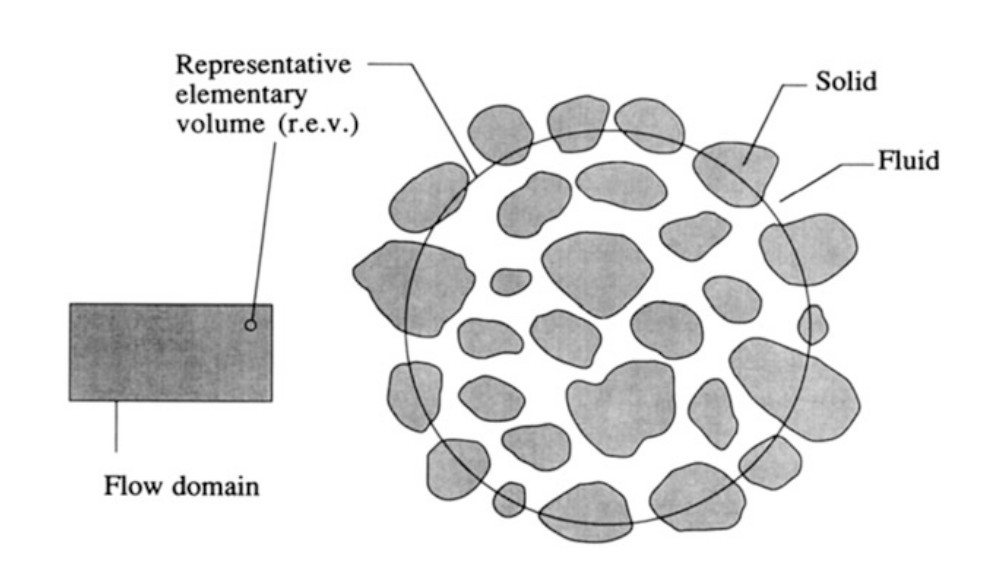
\includegraphics[scale=0.3]{figures/Porous_REV}
\caption{Representation of porous media where the averaging approach is used. From Nield and Bejan}
\end{figure}
\end{center}
\begin{center}
\begin{figure}[!ht]
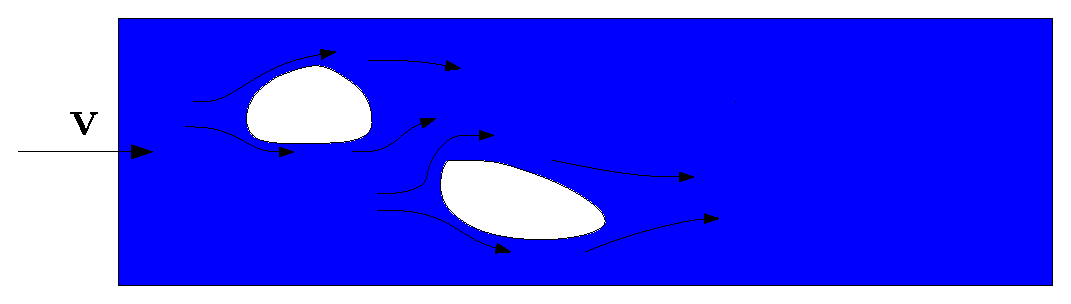
\includegraphics[width=0.9\linewidth]{figures/Porous_Islands}
\caption{River flow around two islands representing the pores. The full Navier-Stokes system should be solved for this problem}
\end{figure}
\end{center}
\subsection{Biot's equations}
The stress tensor for the Biot problem is 
\[ \sigma_s = -pI + 2\mu \epsilon(\mathbf{U}) + \lambda\text{tr}(\epsilon(\mathbf{U}))I  \]
Here $\mu$ and $\lambda$ are Lame's parameters for the solid. The parameter $\alpha = \frac{K}{H}$ is known as the Biot-Willis coefficient. $K$ is known as the drained bulk modulus, and $\frac{1}{K}$ denotes compressibility. $H$ is a poroelastic parameter describing how much the bulk volume changes due to a change in pore pressure while holding the applied stress constant. Again, conservation of momentum and mass, respectively, yields
\begin{align}
	 - \mu \nabla ^2 \mathbf{U}
	 - \lambda \nabla \nabla \cdot \mathbf{U}
	 + \nabla p = \mathbf{F}_v \label{MomentumS}
\end{align}
\begin{align}
	 (\nabla \cdot \mathbf{U})_t
	 - \nabla \cdot (\mu_f^{-1} \mathbf{K} \nabla p) 
	 = 0 \label{ContinuityS}
\end{align}
Where $\mu_f$ is the dynamic viscosity of the fluid and the t-subscript denotes time derivative. As described in \cite{Niel13}, $-\mu^{-1}\mathbf{K} \nabla p$ represents the fluid velocity in the porous medium relative to the solid movement. In other words, the total fluid movement in the poroelastic medium is $\mathbf{U}_t - \mu_f^{-1}\mathbf{K} \nabla p$. $\mathbf{K}$ is known as the permeability matrix. In an isotropic medium we can assume that $\mathbf{K}$ is a scalar constant, $K$.
\\
Equations \eqref{MomentumS}-\eqref{ContinuityS} are nothing more than superpositioning of the tho phases. The material derivatives in \eqref{MomentumS} has been dropped under the assumption that these terms are small. This assumption is known as a quasistatic approximation. 
\\

\section{Descriptions of Motion} \label{sec:DoM}
In the previous section, we saw that the stress tensor for elastic solids were linked to the total displacement from the stress-free configuration of the material. The stresses and velocity in the material will depend on the current deformation of the material with respect to the stress-free configuration. To this end, it will be convenient to provide the reader with two classical descriptions of a continuum in motion. 
\\
\\
\subsection{Lagrangian and Eulerian descriptions of motion}
We consider a domain $\Omega_{\mathbf{X}} \in \mathbb{R}^3$ consisting of material particles $\mathbf{X}$. The domain can undergo deformations, and the deformed domain, $\Omega_{\textit{\textbf{x}}}$, is the current configuration at time $t$. 
\begin{center}
\begin{figure}[!ht]
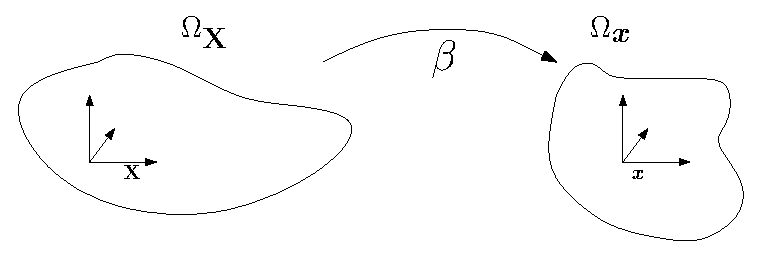
\includegraphics{figures/Lagrangian_domain} \label{Lagrangian}
\caption{Lagrangian description of motion. The mapping $\beta$ maps the reference coordinates to the spatial ones}
\end{figure}
\end{center}

We define the one-to-one mapping:
\begin{align}
\beta \,\, : \,\, \Omega_{\mathbf{X}} \times [0,T] \rightarrow  \Omega_{\mathbf{x}} \times [0,T] \\
(\mathbf{X},t) \rightarrow \beta(\mathbf{X},t) = (\mathbf{x},t)
\end{align}
Which takes any point $\mathbf{X}$ in the reference configuration to a new position $\mathbf{x} = \beta(\mathbf{X},t)$ at time $t$. As the mapping is one-to-one, it is also possible to keep track of the history of the motion by the inverse, $\beta^{-1}$. The time is measured with the same variable, $t$, in both domains. The gradient of $\beta$ with respect to $(\mathbf{X},t)$ can be written in matrix form as:
\begin{align}
\pdi{\beta}{(\mathbf{X},t)} = \begin{pmatrix} \pdi{\mathbf{x}}{\mathbf{X}} & \mathbf{v} \\
											0^T & 1
								\end{pmatrix} \label{betaGradient}
\end{align}
where the material velocity
\begin{align} \mathbf{v}(\mathbf{X},t) = \pdi{\mathbf{x}}{t}\Big{|}_{\mathbf{X}} \label{MatVel}
\end{align}
is the temporal change in the spatial variable $\mathbf{x}$ while holding \textbf{X} fixed. $0^T$ denotes a null vector. 
\\
The \textit{Lagrangian} description, where we follow a fixed set of material particles as suggested by the mapping $\beta$, is often used. In the Lagrangian description all quantities are expressed in terms of the reference configuration $\Omega_{\mathbf{X}}$ and time. In other words, even though the material is deformed, we can still compute displacements and particle velocities using the material coordinates $\mathbf{X}$. For instance, the displacement from the starting material configuration will be given as $\beta(\mathbf{X},t) - \mathbf{X}$ and the velocity as given in \eqref{MatVel}. \\ Because the grid coincides with the material coordinates, there are no convective terms in the Lagrangian description. In the context of Reynold's Transport theorem, the Lagrangian approach coincides with a moving control volume consisting of the same material points at all time. When a material undergoes large deformations or for instance vortices or turbulence occour, the material velocity from the Lagrangian point of view becomes difficult to handle. 
\\
\\
In fluid mechanics the \textit{Eulerian} description is the most used, which means that fluid flows through a fixed region in space and in each point we can measure various properties or quantities such as velocity, pressure and temperature. The conservation equations in the Eulerian description are expressed in terms of the spatial coordinates $\mathbf{x}$ and time, and are neither connected to a reference configuration nor the material coordinates. Compared to the Lagrangian approach, large material deformations is not a problem, as material can enter and leave the fixed domain. This movement of a material through a fixed region results in convective effects, and convection operators can often be problematic in computational fluid dynamics due to their non-symmetric nature. 
\\
\\
\subsection{The Arbitrary Eulerian Lagrangian description}
To be able to couple the Lagrangian approach for the solid with the Eulerian approach for the fluid, we need some referential system, not attached to the material points neither totally fixed in space. This type of description is common in FSI analysis and is known as the \textit{arbitrary Lagrangian-Eulerian} (ALE) description.
\\
\\The following derivation is inspired by the the works on Arbitrary Lagrangian-Eulerian methods by Donea et. al in \cite{Done04}. 
\\
\\
The need for an additional set of coordinates, an independent referential system with reference coordinates $\chi$ is introduced. This introduces two new mappings to relate all the different configurations as shown in fig. 
\begin{center}
\begin{figure}[!ht]
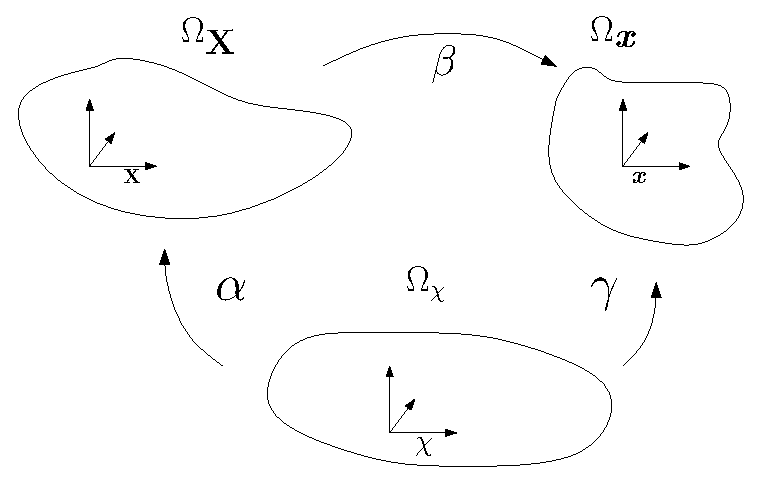
\includegraphics{figures/ALE_domain} \label{ALE_domain}
\caption{The three domains needed in the ALE formulation}
\end{figure}
\end{center}

The mappings are defined similarly to $\beta$ as
\begin{align}
\gamma \,\, : \,\, \Omega_{\chi} \times [0,T] \rightarrow  \Omega_{\mathbf{x}} \times [0,T] \\
(\chi,t) \rightarrow \gamma(\chi,t) = (\mathbf{x},t)
\end{align}
and the gradient of $\gamma$
\begin{align}
\pdi{\gamma}{(\chi,t)} = \begin{pmatrix} \pdi{\mathbf{x}}{\chi} & \mathbf{w} \\
											0^T & 1
								\end{pmatrix} \label{gammaGradient}
\end{align}
In addition, 
\begin{align} \mathbf{w}(\chi,t) = \pdi{\mathbf{X}}{t}\Big{|}_{\chi} \label{MeshVel}
\end{align}
denotes the mesh velocity. Both the mesh and the material can move independently of the laboratory. More precise, relative to some referential point in space, the fluid moves with veloctiy $\mathbf{v}$ and the domain moves with velocity $\mathbf{w}$. 
\\
\\
To complete the relation between the different velocities, we define the inverse of $\alpha$ directly: 
\begin{align}
\alpha^{-1} \,\, : \,\, \Omega_{\mathbf{X}} \times [0,T] \rightarrow  \Omega_{\chi} \times [0,T] \\
(\mathbf{X},t) \rightarrow \alpha^{-1}(\mathbf{X},t) = (\chi,t)
\end{align}
The gradient is given as
\begin{align}
\pdi{\alpha^{-1}}{(\mathbf{X},t)} = \begin{pmatrix} \pdi{\chi}{\mathbf{X}} & \mathbf{\hat{v}} \\
											0^T & 1
								\end{pmatrix} \label{alpha_Gradient}
\end{align}
Where the velocity 
\begin{align} \mathbf{\hat{v}}(\mathbf{X},t) = \pdi{\chi}{t}\Big{|}_{\mathbf{X}} \label{HatVel}
\end{align}
denotes the temporal change in the referential system while holding the material particle $\mathbf{X}$ fixed. Therefore the velocity $\mathbf{\hat{v}}$ can be interpereted as the particle velocity in the referential domain. \\
\\
We use that $\beta = \gamma \, \circ \, \alpha^{-1} = \gamma(\alpha^{-1}(\mathbf{X},t))$ and obtain a relation between the different velocities by differentiating $\beta$. 
\begin{align}
\pdi{\beta}{(X,t)}(\mathbf{X},t) & = \pdi{\gamma}{(\chi,t)}(\alpha^{-1}(\mathbf{X,t}))\, \pdi{\alpha^{-1}}{(\mathbf{X},t)}(\mathbf{X},t) \\
& = \pdi{\gamma}{(\chi,t)}(\chi,t)\, \pdi{\alpha^{-1}}{(\mathbf{X},t)}(\mathbf{X},t)
\end{align}
In matrix form this equation is written:
\begin{align}
	\begin{pmatrix} \pdi{\mathbf{x}}{\mathbf{X}} & \mathbf{v} \\
											0^T & 1
	\end{pmatrix} 
	= 
	\begin{pmatrix} \pdi{\mathbf{x}}{\chi} & \mathbf{w} \\
											0^T & 1
	\end{pmatrix}
	\begin{pmatrix} \pdi{\chi}{\mathbf{X}} & \mathbf{\hat{v}} \\
											0^T & 1
	\end{pmatrix}
\end{align}
After block-multiplication of the right hand side we end up with an equation relating all the different velocities:
\begin{align}
\mathbf{v} = \pdi{\mathbf{x}}{\chi}\cdot \mathbf{\hat{v}} + \mathbf{w}
\end{align}
To this end, it is convenient to define the convective velocity
\begin{align}
\mathbf{c}:= \mathbf{v}-\mathbf{w} = \pdi{\mathbf{x}}{\chi}\cdot \mathbf{\hat{v}}
\end{align}
which is the relative velocity between the material and the mesh. 
\\
\\
To obtain relation between quantities to formulate the balance equations, we let a scalar quantity, $Q$ be defined as $Q(\mathbf{x},t), Q^*(\chi,t)$ and $Q^{**}(\mathbf{X},t)$ in the spatial, referential and material domains respectively. \\
\\
To obtain a relation between the spatial description, $Q$, and material description $Q^{**}$ we can utilize the previously described mapping $\beta$:

\begin{align}
Q^{**}(\mathbf{X},t) = Q(\beta(\mathbf{X},t),t) = Q \, \circ \, \beta
\end{align}

The gradient of $Q^{**}$ can then be computed as
\begin{align}
\pdi{Q^{**}}{(\mathbf{X},t)}(\mathbf{X},t) = \pdi{Q}{(\mathbf{x},t)}(\mathbf{x},t) \, \pdi{\beta}{(\mathbf{X},t)}(\mathbf{X},t)  \label{Grad_Q}
\end{align}

\begin{align}
	\begin{pmatrix} \pdi{Q^{**}}{\mathbf{X}} & \pdi{Q^{**}}{t}
	\end{pmatrix}
	= 
	\begin{pmatrix} \pdi{Q}{\mathbf{x}} & \pdi{Q}{t}
	\end{pmatrix}
	\begin{pmatrix} \pdi{\mathbf{x}}{\mathbf{X}} & \mathbf{v} \\
											0^T & 1
	\end{pmatrix} \label{Matrix_Q}
\end{align}
After multiplication one can obtain the well known equation between material and spatial time derivaties:
\begin{align}
\pdi{Q^{**}}{t} = \pdi{Q}{t} + \pdi{Q}{\mathbf{x}} \cdot \mathbf{v} \label{Mat_Spa}
\end{align}
To ease notation we now recognize the material and spatial time derivatives $\pdi{Q^{**}}{t} = \pdi{Q}{t}\Big{|}_{\mathbf{X}}$, $\pdi{Q}{t} = \pdi{Q}{t}\Big{|}_{\mathbf{x}}$, and define the material and spatial derivatives the following way
\begin{align}
\frac{\mathrm{d}}{\mathrm{dt}} := \pdi{}{t}\Big{|}_{\mathbf{X}} \hspace{3cm} \pdi{}{t} := \pdi{}{t}\Big{|}_{\mathbf{x}}
\end{align}
The relation \eqref{Mat_Spa} can now be written in a form probably already known to the reader
\begin{align}
\frac{\mathrm{d}Q}{\mathrm{dt}} = \pdi{Q}{t} + \mathbf{v} \cdot \nabla Q \label{Material_derivative}
\end{align}
The next step is to relate the material and the referential description of the quantity, $Q^{**}$ and $Q^*$ respectively, by the mapping $\alpha$. This relation is written as 
\begin{align}
Q^{**} = Q^* \, \circ \, \alpha^{-1}
\end{align}
By proceeding the exact same way as way as in \eqref{Grad_Q} and \eqref{Matrix_Q} the relation between material and referential time derivatives is written
\begin{align}
\pdi{Q^{**}}{t} = \pdi{Q^*}{t} + \pdi{Q^*}{\chi}\cdot \mathbf{\hat{v}}
\end{align}
If we rather want to express the spatial derivative of $Q^*$ in the spatial domain, we can use the definition of $\mathbf{\hat{v}}$ from \eqref{HatVel} to end up with
\begin{align}
\pdi{Q^{**}}{t} = \pdi{Q^*}{t} + \pdi{Q}{\mathbf{x}} \cdot \mathbf{c}
\end{align}
This equation can be written in more common notation, and the following is known as \textit{The fundamental ALE equation}
\begin{align}
\frac{\mathrm{d}Q}{\mathrm{dt}} = \pdi{Q}{t}\Big{|}_{\chi} + \mathbf{c} \cdot \nabla Q \label{Fundamental_ALE}
\end{align}
and states that the time derivative in the material configuration equals its local (referential) derivative plus a convective term taking into account the relative difference in velocity between the two systems. It should be noted that the relations presented also holds for vector quantities. 
\\
\\
Also, by combining equations \eqref{Material_derivative} and \eqref{Fundamental_ALE}, we can relate the spatial time derivative with the referential time derivative as
\begin{align}
\pdi{Q}{t} = \pdi{Q}{t}\Big{|}_{\chi} - \mathbf{w} \cdot \nabla Q \label{Spatial_referential}
\end{align}



\section{Balance equations in the ALE framework}
To obtian appropriate balance equations in the ALE framework we start by noting that the balance equations can be written in terms of the material derivates as
\begin{align}
\frac{\mathrm{d}\rho}{\mathrm{dt}} = \pdi{\rho}{t} + \mathbf{v} \cdot \nabla \rho= -  \rho \cdot \nabla \mathbf{v}
\end{align}
\begin{align}
\rho \frac{\mathrm{d}\mathbf{v}}{\mathrm{dt}} = \rho \Big{(} \pdi{\mathbf{v}}{t} + (\mathbf{v} \cdot \nabla ) \mathbf{v} \Big{)} = \nabla \cdot \sigma
\end{align}
By using \eqref{Spatial_referential}, the spatial time derivatives can be replaced to obtain equations for the ALE framework:
\begin{align}
\pdi{\rho}{t}\Big{|}_\chi + \mathbf{c} \cdot \nabla \rho= -  \rho \cdot \nabla \mathbf{v}
\end{align}
\begin{align}
\rho \Big{(} \pdi{\mathbf{v}}{t}\Big{|}_\chi + (\mathbf{c} \cdot \nabla ) \mathbf{v} \Big{)} = \nabla \cdot \sigma
\end{align}
Which shows that all one have to do in order to transform the Eulerian form of the balance equations into the ALE formulation is to replace the convective velocity with the relative velocity between the material and the mesh. 
\subsection{Mesh updating}
The velocity $\mathbf{w}$ can be seen as the mesh velocity when a computational mesh is used. In FSI, the ALE framework provides flexibility to combine the Lagrangian and Eulerian descriptions of motion. On the structural part, as well as on the fluid-structure interface we take a Lagrangian approach. The domain $\Omega_s$ consists of the same material particles at all times and moves exactly with the material points within the structure. That is, $\mathbf{v}_s = \mathbf{w}_s$. The fluid domain has to follow the changes on the fluid-structure interface. Other than that the mesh velocity in the fluid domain is arbitrary in principle, but the choice of mesh velocity in the fluid domain is important for the accuracy of the solver. In general, important aspects to consider is disortion and squeeze of each element in the fluid domain. \\
\\
A Laplacian smoothing algorithm is used to update the mesh, consisting of solving a Laplace (or Poisson) equation for the mesh displacement in the fluid. The method is a mesh regularization method where the lines in the mesh have equal potential. This method was first introduced by Winslow in 1963 \cite{Wins63}.
\section{Fluid Structure Interaction}
In the case of an Newtonian incompressible fluid the mathematical problem consists of solving
\begin{align}
\begin{rcases}
\rho \Big{(} \pdi{\mathbf{v}}{t} + ((\mathbf{v}-\mathbf{w})  \cdot & \nabla )  \mathbf{v} \Big{)}  =   \nabla \cdot \sigma_f(\mathbf{v},p)  \\
& \nabla \cdot \mathbf{v} \, = 0 \\
& \nabla ^2 \mathbf{U} \, = 0
\end{rcases}
& \text{ in } \Omega_f^t \\ \\
\begin{rcases}
\rho \pdi{\mathbf{v}}{t}  = &  \nabla \cdot \sigma_s(\mathbf{U}) \\
\mathbf{w} =  \mathbf{v}
\end{rcases}& \text{ in } \Omega_s^t 
\end{align}
In the case of fluid interacting with a solid structure, no material can cross the moving boundary and thus the fluid and solid velocity must be equal on the interface between the fluid and the solid. In general, one have to ensure mass conservation on the boundary. In addition the forces acting on the surface must be equal. A difference in forces from each material on the interface would result in infinite acceleration on the infinitely thin surface. Mathematicly, these two conditions can be stated as
\begin{align}
\begin{rcases}
\sigma_f \cdot \mathbf{n} & =  \sigma_s \cdot \mathbf{n} \\
\mathbf{v}_f & = \mathbf{v}_s
\end{rcases}
\text{ on } \Gamma^t
\end{align}
And will be used at all interfaces in FSI simulations. Kinematic or dynamic boundary conditions will be needed on the other boundaries as well, but will differ depending on the problem considered. 
\\


